\chapter{Цель и задачи}
\label{ch:intro}

\section*{\textbf{Цель:}} 

Моделирование поведения системы массового
обслуживания. Сравнение аналитических и статистических оценок
стационарных характеристик для различных видов управляющих
последовательностей.

\section*{Задание к лабораторной работе}

\begin{figure}[H]
    \centering
    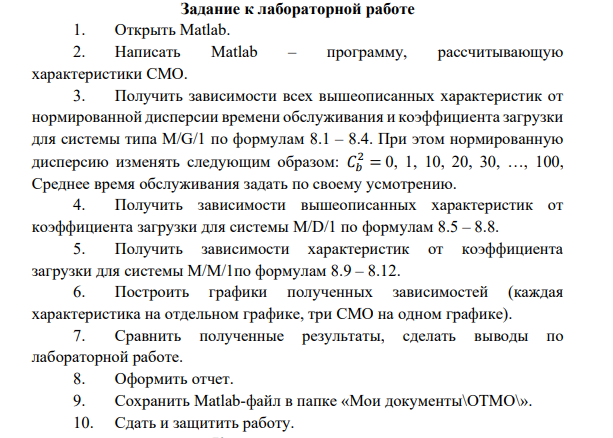
\includegraphics[width=1.0\textwidth]{task.png}
    \caption{Задание для лабораторной работы}
\end{figure}


\endinput